\section{Visualization Approach}
\label{sec:solution}

\subsection{Probe Clustering Visualization}
\label{sec:probe}

As was discussed before in the Section~\ref{sec:dataset_description} cluster analysis result graph is binary tree.

,,A binary tree is a connected acyclic graph such that the degree of each vertex is no more than 3. A rooted binary tree is such a graph that has one of its vertices of degree no more than 2 singled out as the root. With the root thus chosen, each vertex will have a uniquely defined parent, and up to two children; however, so far there is insufficient information to distinguish a left or right child. If we drop the connectedness requirement, allowing multiple connected component in the graph, we call such a structure a forest"~\cite{BINARY_TREE} Simple binary tree showed on the Figure~\ref{fig:simple_binary_tree}

\begin{figure}[h!]
\centering
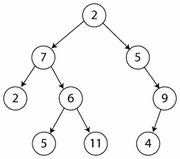
\includegraphics[scale=1.0]{pictures/simple_binary_tree.png}
\caption{A simple binary tree graph}
\label{fig:simple_binary_tree}
\end{figure}

There are several visualization methods for binary trees and more specific methods for cluster results. The main method for visualizing clusters is a -- dendrogram. Here is sample dendrogram visualization on the Figure~\ref{fig:dendrogram_1} produced by MATLAB 7.2.

\begin{figure}[h!]
\centering
\subfloat[Dendrogram]{
    \label{fig:dendrogram_1}
    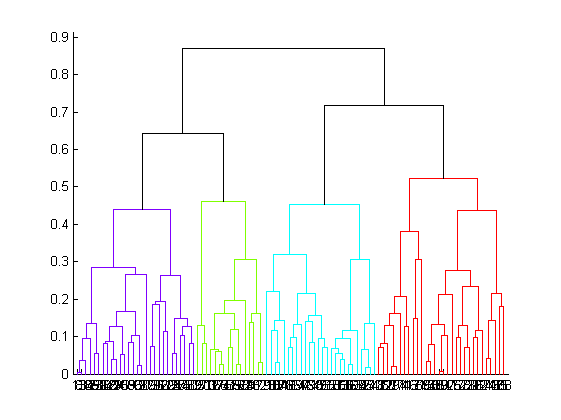
\includegraphics[scale=0.45]{pictures/dendrogram.png}
}
\subfloat[Polar Dendrogram]{
    \label{fig:polardendrogram}
    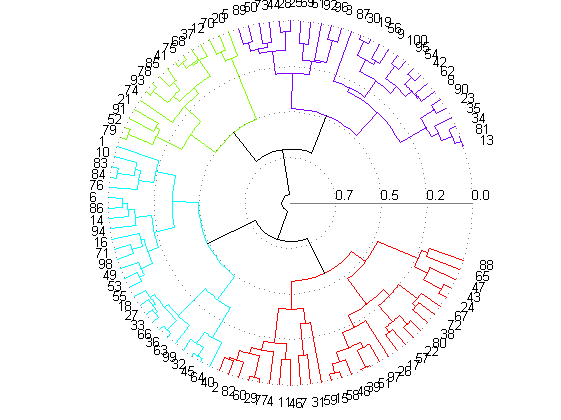
\includegraphics[scale=0.45]{pictures/polardendrogram.png}
}
\label{fig:dendrograms}
\caption{Cluster visualisations}
\end{figure}


Figure~\ref{fig:polardendrogram} shows a polar dendrogram visualization algorithm of the same cluster tree produced by MATLAB.

One of the main ideas was to use polar dendrogram algorithm for cluster visualization. The Figure~\ref{fig:JUNG_radial_layout} shows visualization of the Cluster using native JUNG radial layout algorithm. Red are nodes and white is edges, black is background. As picture shows algorithm doesn't count nature of the cluster: very deep binary tree not wide as it is common for cluster analysis results, that's why it has many edge overlapping.


\begin{figure}[h!]
\centering
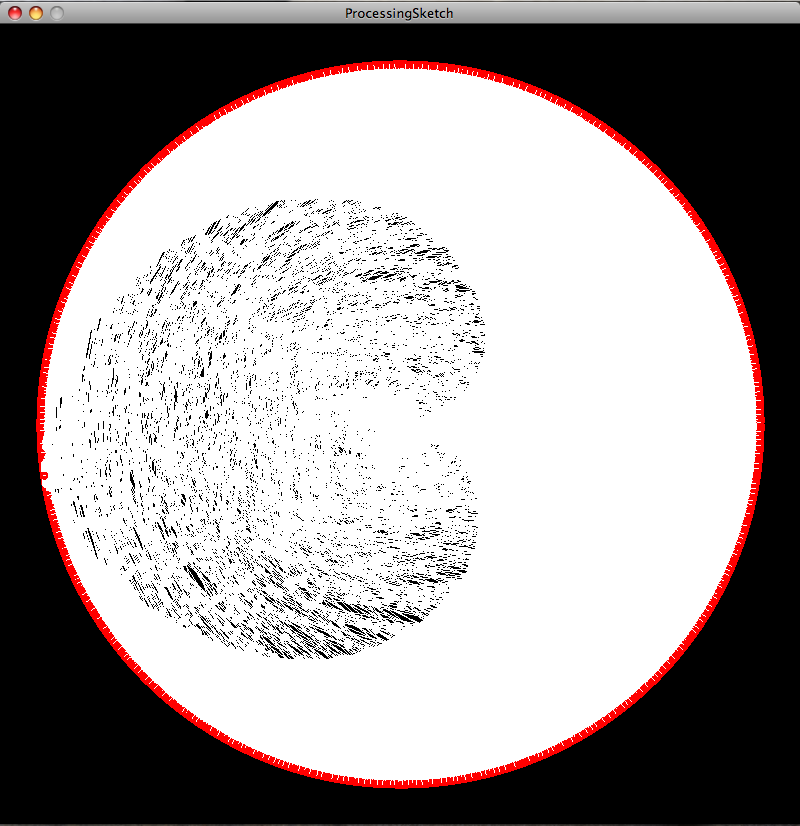
\includegraphics[scale=0.4]{pictures/using_JUNG_radial.png}
\caption{Cluster visualization using JUNG radial layout}
\label{fig:JUNG_radial_layout}
\end{figure}


Also to visualization issue it has performance issue -- without any measurement was seen for an eye that program does not allow smooth interaction. Low performance issue was in nature of the visualization in the JUNG: it uses very complex hierarchical structure with many utility classes per visualized object and the cost is big memory usage. Also JUNG uses Java 2D~\cite{JAVA_2D} which by itself is `heavyweight' because it's part of the Java AWT -- Abstract Windows Toolkit.


,,The Abstract Window Toolkit (AWT) is Java's original platform-independent windowing, graphics, and user-interface widget toolkit. The AWT is now part of the Java Foundation Classes (JFC) the standard API for providing a graphical user interface (GUI) for a Java program. When Sun Microsystems first released Java in 1995, AWT widgets provided a thin level of abstraction over the underlying native user interface. For example, creating an AWT check box would cause AWT directly to call the underlying native subroutine that created a check box."~\cite{JAVA_AWT} This technology is outdated and replaced by Swing.


,,Swing is the primary Java GUI widget toolkit. It is part of Sun Microsystems' Java Foundation Classes (JFC) an API for providing a graphical user interface (GUI) for Java programs.
Swing was developed to provide a more sophisticated set of GUI components than the earlier Abstract Window Toolkit. Swing provides a native look and feel that emulates the look and feel of several platforms, and also supports a pluggable look and feel that allows applications to have a look and feel unrelated to the underlying platform."~\cite{JAVA_SWING}


,,Since early versions of Java, a portion of the Abstract Window Toolkit (AWT) has provided platform-independent APIs for user interface components. In AWT, each component is rendered and controlled by a native peer component specific to the underlying windowing system.
By contrast, Swing components are often described as lightweight because they do not require allocation of native resources in the operating system's windowing toolkit. The AWT components are referred to as heavyweight components."~\cite{JAVA_SWING} More detail comparison can be found here.~\cite{AWT_VS_SWING}


The Figure~\ref{fig:cluster_jogl_impl} shows improved JUNG radial algorithm and own visualization implementation using JOGL. JOGL will be discussed in the Section~\ref{sec:opengl}.


\begin{figure}[h!]
\centering
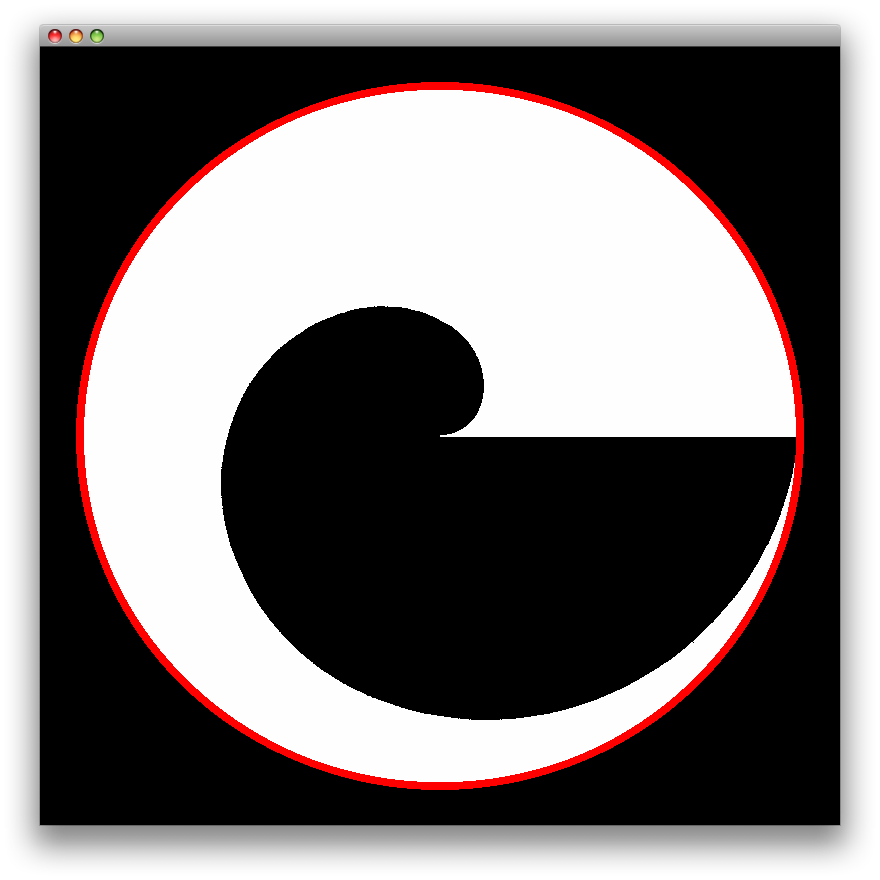
\includegraphics[scale=0.4]{pictures/cluster_jogl_impl.png}
\caption{Cluster visualization using JOGL and improved JUNG radial layout}
\label{fig:cluster_jogl_impl}
\end{figure}


The Figure~\ref{fig:cluster_jogl_impl_with_subgraph_1} and Figure~\ref{fig:cluster_jogl_impl_with_subgraph_2} shows cluster visualization and highlighted subgraph (subgraph extraction algorithm was discussed in the Section~\ref{sec:problem}). This pictures show the nature of the dataset. Improved version has good performance and better visualization but still has issues: there are too many elements in the scene, it is impossible to identify separate gene or trace highlighted graph genes.

\begin{figure}[h!]
\centering
\subfloat[Cluster graph and highlighted subgraph]{
    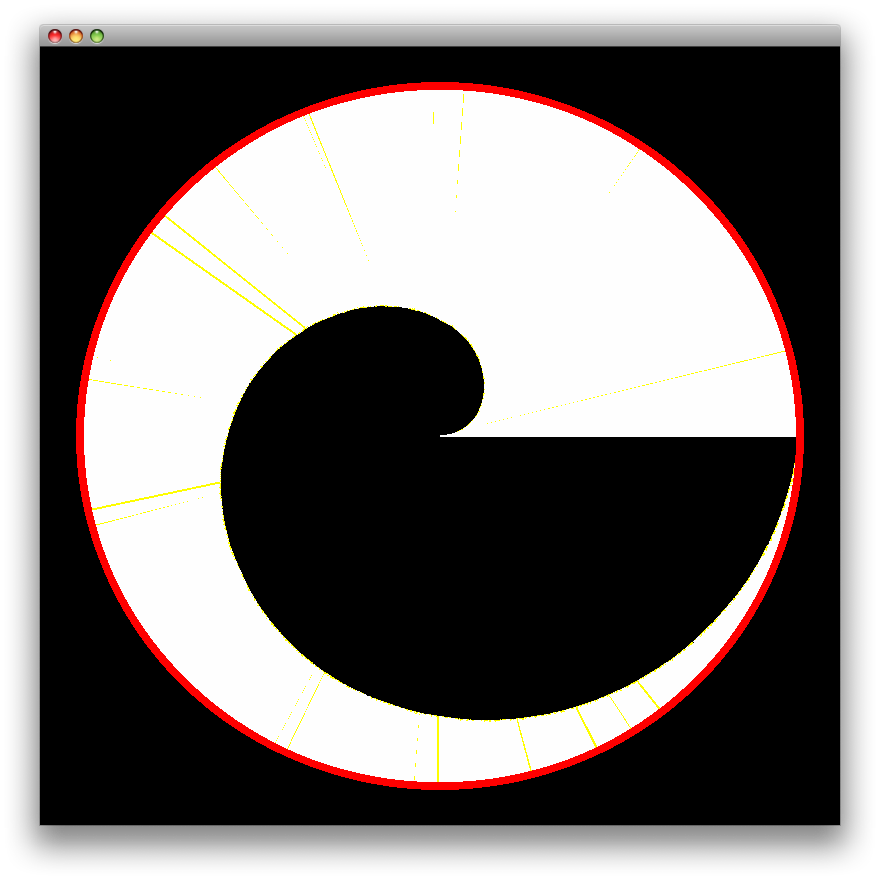
\includegraphics[scale=0.2]{pictures/cluster_jogl_impl_with_subgraph_1.png}
    \label{fig:cluster_jogl_impl_with_subgraph_1}
}
\subfloat[Cluster graph and highlighted subgraph]{
    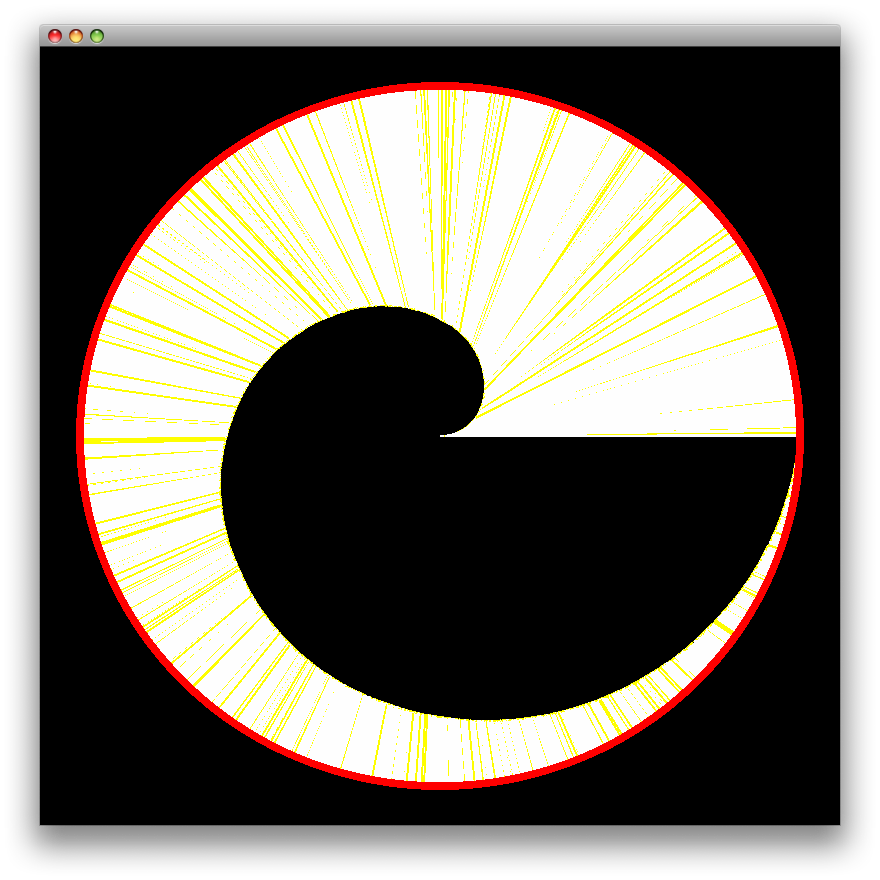
\includegraphics[scale=0.2]{pictures/cluster_jogl_impl_with_subgraph_2.png}
    \label{fig:cluster_jogl_impl_with_subgraph_2}
}
\caption{Cluster graph visualisation using improved JUNG polar dendrogram layout}
\end{figure}


%%%%%%%%%%%%%%%%%%%%%%%%%%%%%%%%%%%%%%%%%%%%%%%%%%%%%%%%%%%%%%%%%%%%%%%%%%%%%%%%%%%%%%%%%%%%%%%%%%%%
% cluster visualization explanation
\subsection{Cluster Analysis Results Visualization}
\label{sec:cluster}

Figure~\ref{fig:Cytoscape_Cluster_2} from Section~\ref{sec:dataset_description} shows cluster graph specific structure: it is very high, unbalanced and has not so deep sub-parts. It is possible to use this disadvantage as advantage and abstract sub-parts to reduce drawing area. Extract those nodes and edges that form the longest path of the cluster graph - ,,backbone''. Figure~\ref{fig:cluster_visualisation} shows algorithm work step by step. Backbone vertices are filled with yellow and showed in Figure~\ref{fig:cluster_visualisation_algorithm_1}. Next step is to abstract branches into groups, group size is scaled according to amount of elements inside.

\begin{figure}[h!]
\centering
\subfloat[Backbone and branches]{
    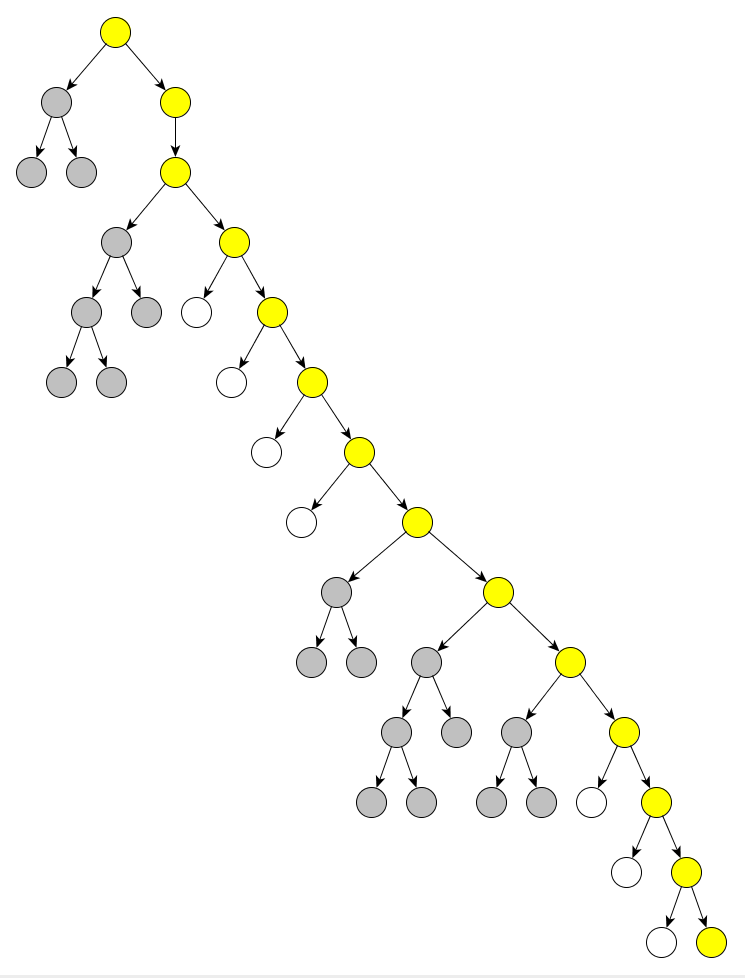
\includegraphics[scale=0.15]{pictures/cluster_visualisation_algorithm_1.png}
    \label{fig:cluster_visualisation_algorithm_1}
}
\subfloat[Abstract branches into groups]{
    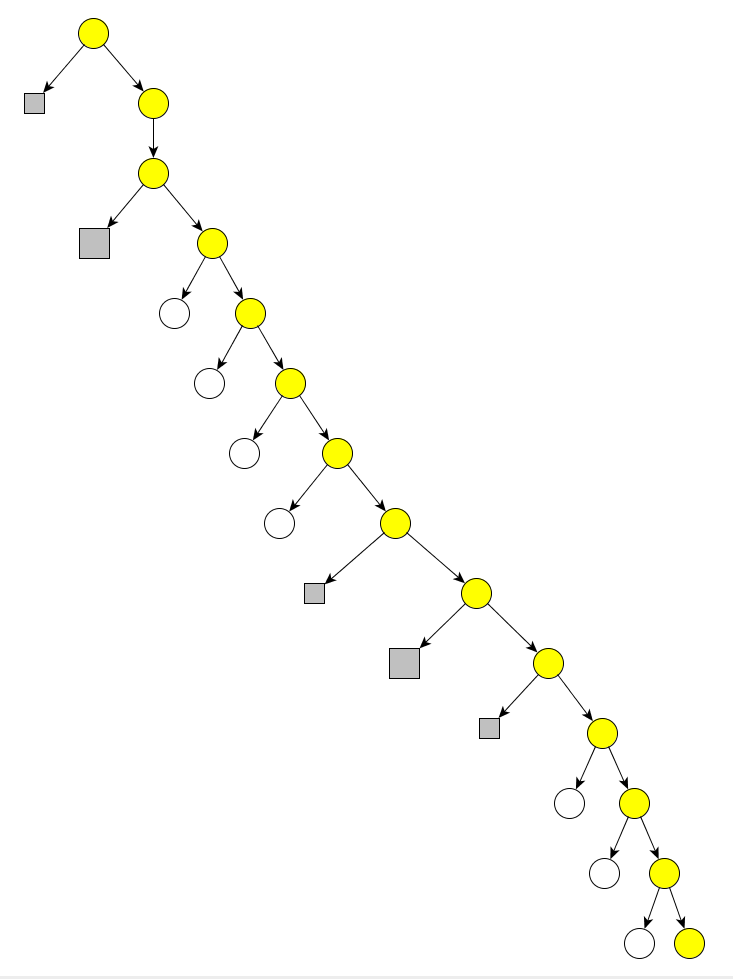
\includegraphics[scale=0.15]{pictures/cluster_visualisation_algorithm_2.png}
    \label{fig:cluster_visualisation_algorithm_2}
}
\subfloat[Scale group size]{
    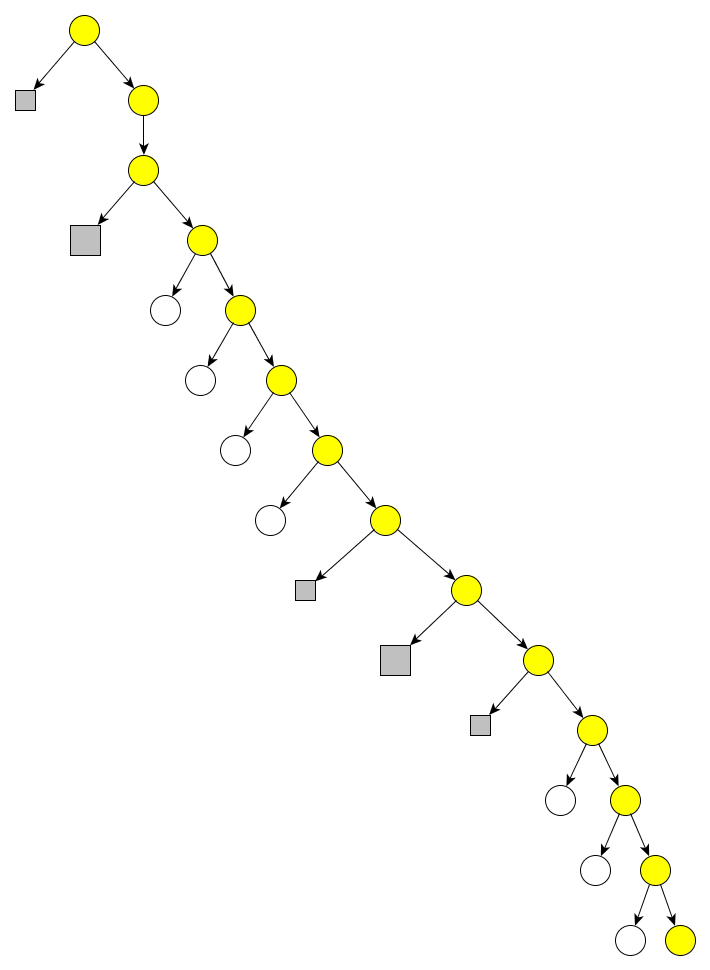
\includegraphics[scale=0.15]{pictures/cluster_visualisation_algorithm_3.png}
    \label{fig:cluster_visualisation_algorithm_3}
}
\caption{Cluster Visualization algorithm}
\label{fig:cluster_visualisation_algorithm}
\end{figure}

The last step is to represent backbone as a spiral, thus preserving space and giving us a possibility to show the complete tree in one view. Figure~\ref{fig:cluster_visualisation_algorithm_4} shows how this approach works.

\begin{figure}[h!]
\centering
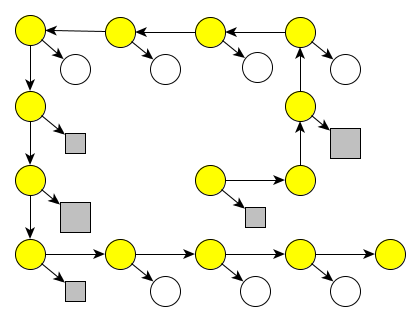
\includegraphics[scale=0.5]{pictures/cluster_visualisation_algorithm_4.png}
\caption{,,Rectangular Spiral Layout''}
\label{fig:cluster_visualisation_algorithm_4}
\end{figure}

Then backbone formed as rectangular spiral with a root in the center and moving in clockwise direction. Figure~\ref{fig:cluster_spiral_visualisation} shows complete visualization result for real cluster tree. This will have to reuse space as much as possible and still gives overview of location of the highlighted vertices in cluster hierarchy -- how far from a root.

\begin{figure}[h!]
\centering
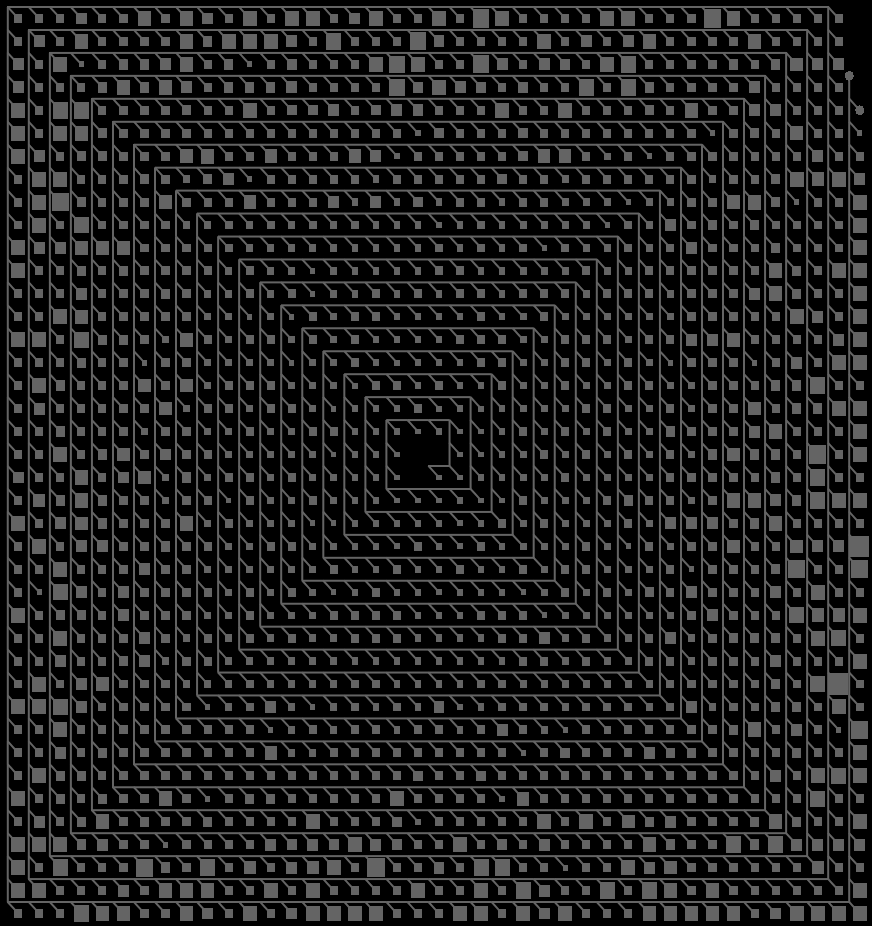
\includegraphics[scale=0.4]{pictures/cluster_spiral_visualisation.png}
\caption{Rectangular spiral Cluster graph visualization}
\label{fig:cluster_visualisation}
\end{figure}

It is possible to explore sub-part (rectangles) of the Cluster graph using lens. User can interactively choose any sub-part and lens with inner content will appear. There are two different lens layouts: polar~\ref{fig:lens_polar} and HV-tree~\ref{fig:lens_tree}. Polar lens layout is based on algorithm used for initial visualization of the Cluster graph explained earlier in Section~\ref{sec:probe}. Both implementations are own made and are not based on any third party source code.

\begin{figure}[h!]
\centering
\subfloat[Polar lens layout]{
    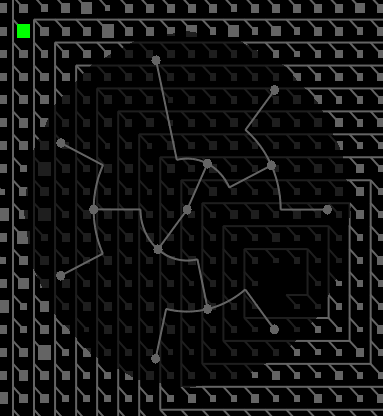
\includegraphics[scale=0.5]{pictures/lens_polar.png}
    \label{fig:lens_polar}
}
\\
\subfloat[HV-tree lens layout]{
    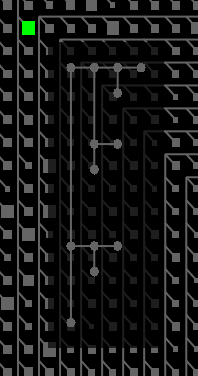
\includegraphics[scale=0.5]{pictures/lens_tree.png}
    \label{fig:lens_tree}
}
\caption{Different lens layouts}
\end{figure}


%%%%%%%%%%%%%%%%%%%%%%%%%%%%%%%%%%%%%%%%%%%%%%%%%%%%%%%%%%%%%%%%%%%%%%%%%%%%%%%%%%%%%%%%%%%%%%%%%%%%


%%%%%%%%%%%%%%%%%%%%%%%%%%%%%%%%%%%%%%%%%%%%%%%%%%%%%%%%%%%%%%%%%%%%%%%%%%%%%%%%%%%%%%%%%%%%%%%%%%%%
% gene ontology visualization explanation
\subsection{Gene Ontology Visualization}
\label{sec:go}

Gene Ontology graph is a directed acyclic graph and highly connected: 24,153 edges and 10,041 vertices, where 3,918 are unconnected components.
Figure~\ref{fig:go_connections_yEd} shows how extremely connected the graph is, the picture was produced by yEd graph editing tool.

\begin{figure}
\centering
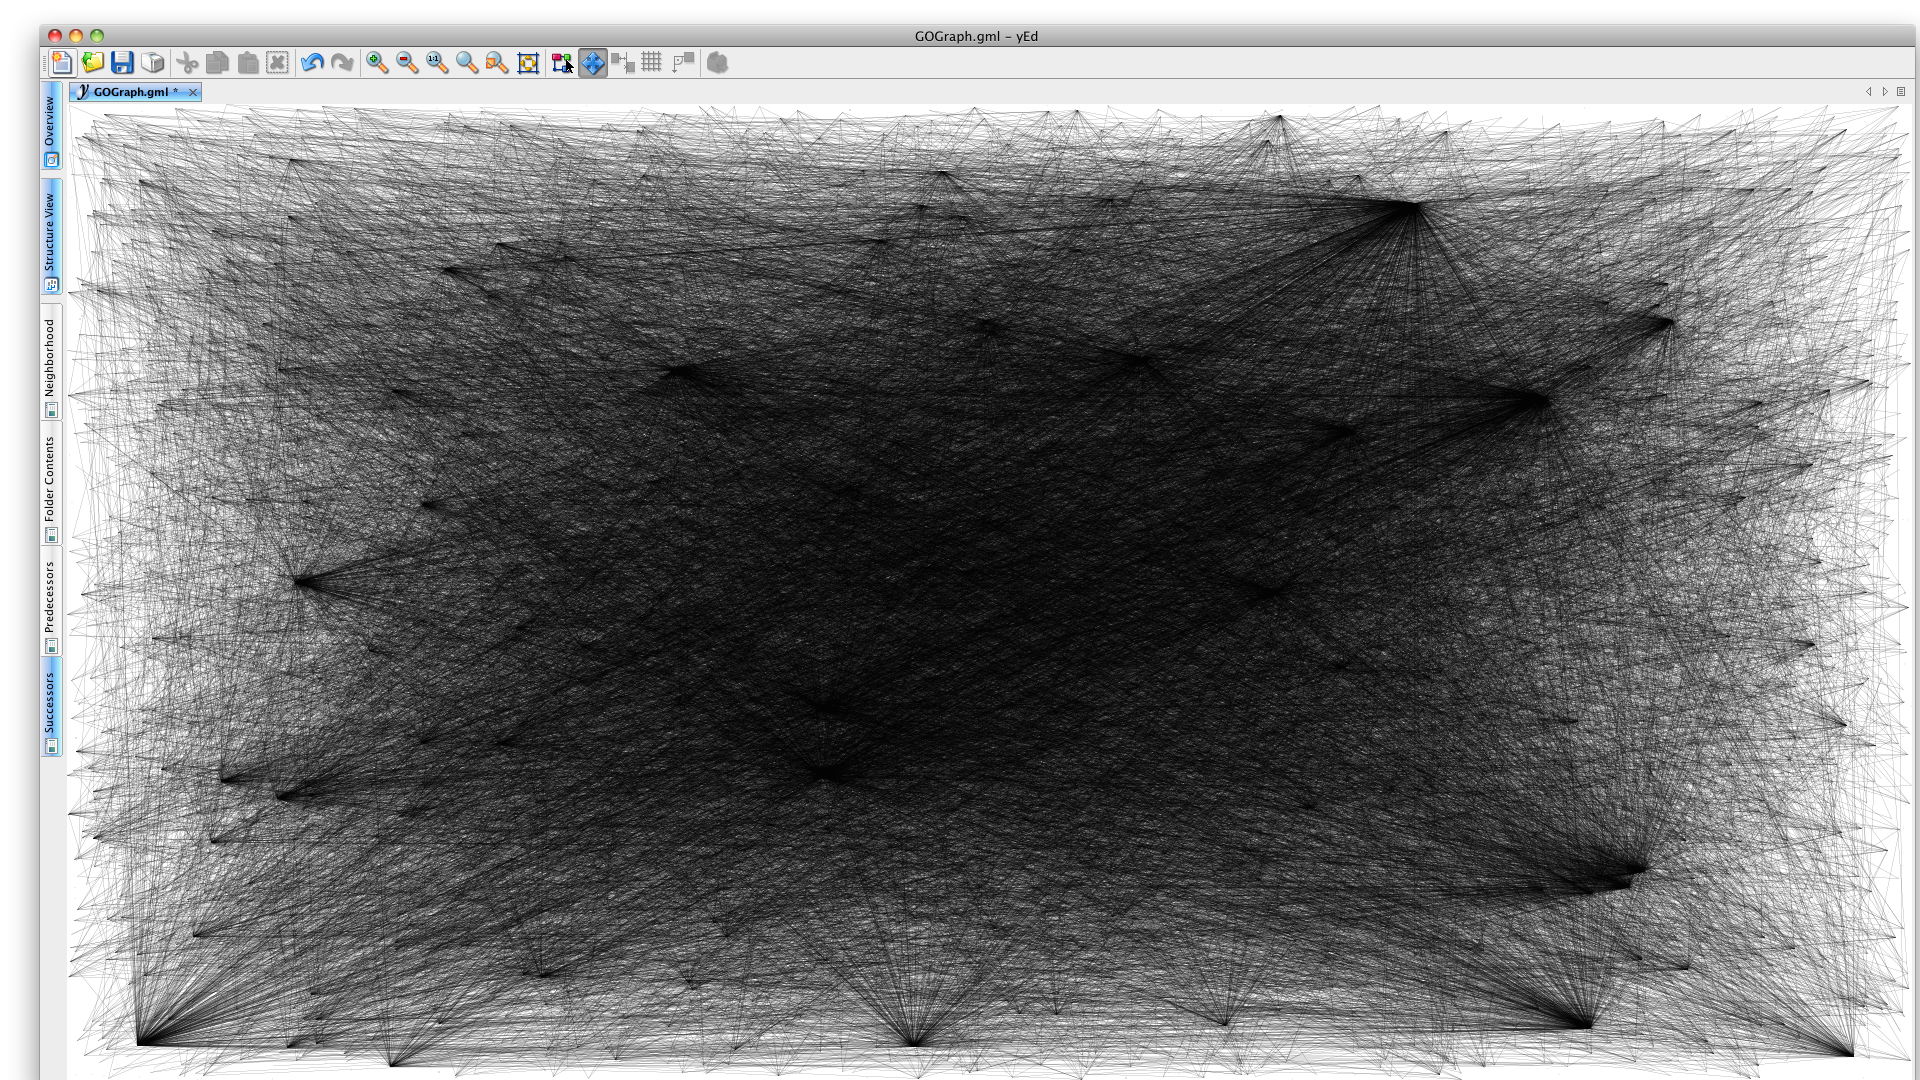
\includegraphics[scale=0.2]{pictures/yEd_GO_2.png}
\caption{Gene Ontology graph visualization using yEd}
\label{fig:go_connections_yEd}
\end{figure}

The high connectivity between elements in the source graph makes it very complicated to explore. Provided visualization approach has several goals.
The first goal is to reduce amount of connections between vertices by showing edges only for ``current'' sub-graph.
It allows to see where the sub-graph is aligned in the whole graph and, in the same time, helps to track its inner structure.
Second goal is an ability to switch from working with genes of the GO graph to discovering relations between GO and Cluster graphs.
For this purpose there are two view modes for GO graph:

\begin{itemize}
   \item levels overview --- show graph levels from top to bottom with corresponding content as ``preview'';
   \item zoomed view --- visualizes only on three levels at the same time in order to focus on genes inside;
\end{itemize}

The last but not least goal is to explicitly show nodes and leafs. Each level is divided into two sections where leafs are red colored on the left and node genes are on the right and having white color.
Color schema can be changes through the settings menu but not leafs-nodes location.
This feature gives further insight into the topology of a specific layer by gaining information about the distribution of leafs and nodes on a particular layer.

There are two layout implementations based on the goals discussed before. First GO layout is ``Levels Layout'' and is shown in Figure~\ref{fig:go_levels_layout}.
Genes are ordered by layers depending on their graph-theoretic distance from the root.

\begin{figure}[h!]
\centering
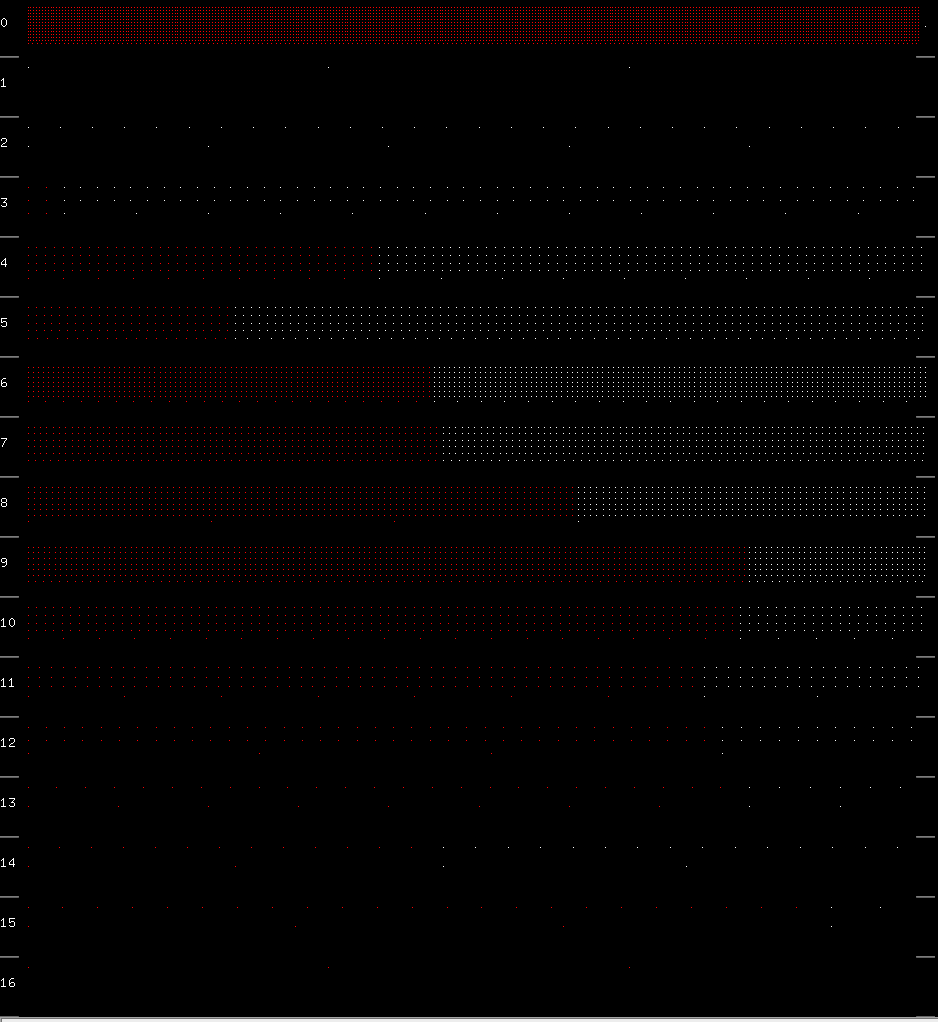
\includegraphics[scale=0.3]{pictures/go_levels_layout.png}
\caption{Gene Ontology Levels Layout visualisation}
\label{fig:go_levels_layout}
\end{figure}

Figure~\ref{fig:go_levels_layout_zoomed} displays the situation when the user zooms in the view.
Although the resulting visualization looks like bar charts, the number of leafs cannot be precisely compared between different layers since
the area the red node pixels (leafs) cover is not proportional to the total number of leafs in each layer.
However, it is proportional to the sum of nodes in that particular layer. In other words, the covered area depends on the specific layer density.
There are unconnected components in the Gene Ontology graph.
Unconnected nodes are placed in the top layer number --- zero. There is an option to show-hide unconnected components from the main menu.
The spatial arrangement of the node pixels within a layer, except the placing of leafs and nodes are in specific regions, is random.

\begin{figure}[h!]
\centering
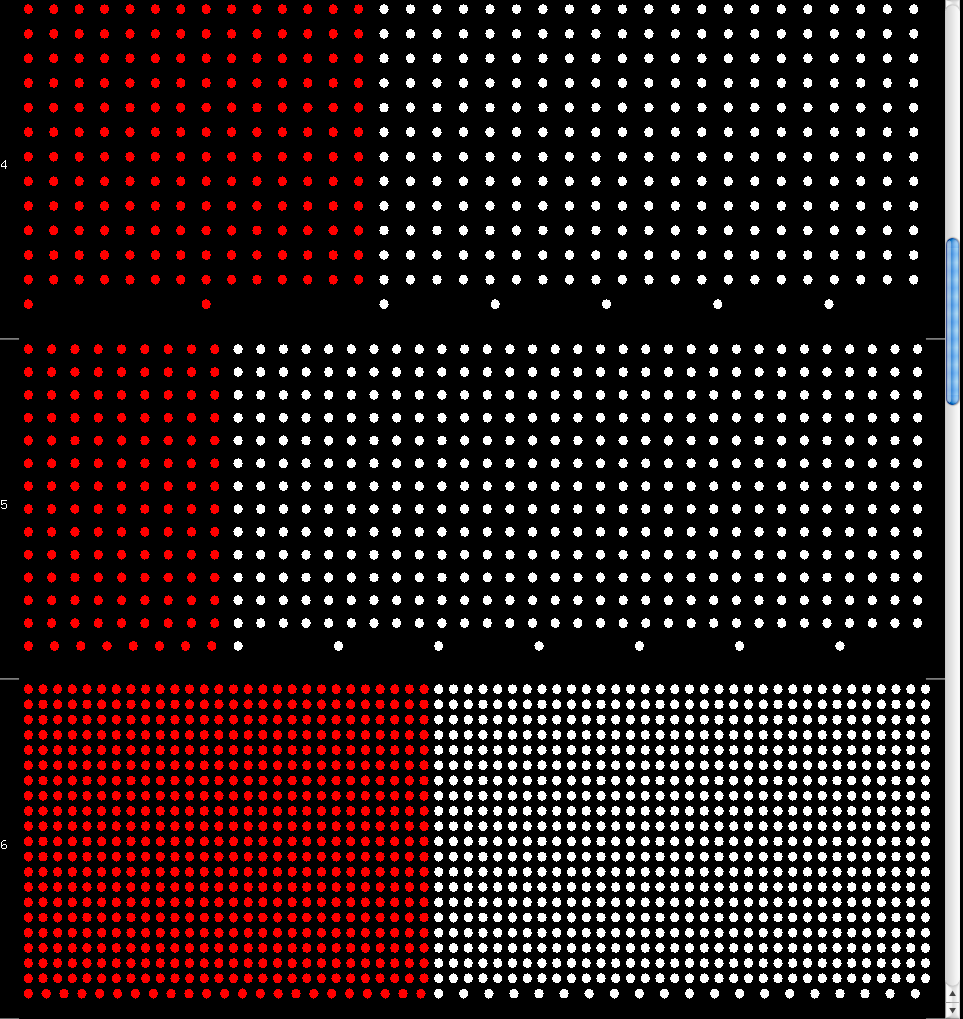
\includegraphics[scale=0.3]{pictures/go_levels_layout_zoomed.png}
\caption{Zoomed view}
\label{fig:go_levels_layout_zoomed}
\end{figure}

Second layering approach ``Leaves Bottom Layout''
(Figure~\ref{fig:go_leaves_bottom_layout}) is similar to the first one in terms of placing the nodes into corresponding layers based on the distance
from the source node and random distribution of the node pixels within each layer.
However, all leafs are placed into one single layer together with unconnected nodes at the bottom of the GO view, i. e., in the layer with the highest number.
Unconnected nodes can be filtered out if necessary. This approach gives insight into the distribution of nodes among different layers without the distraction of the leafs,
thus enriching the perception of the graph topology.

\begin{figure}[h!]
\centering
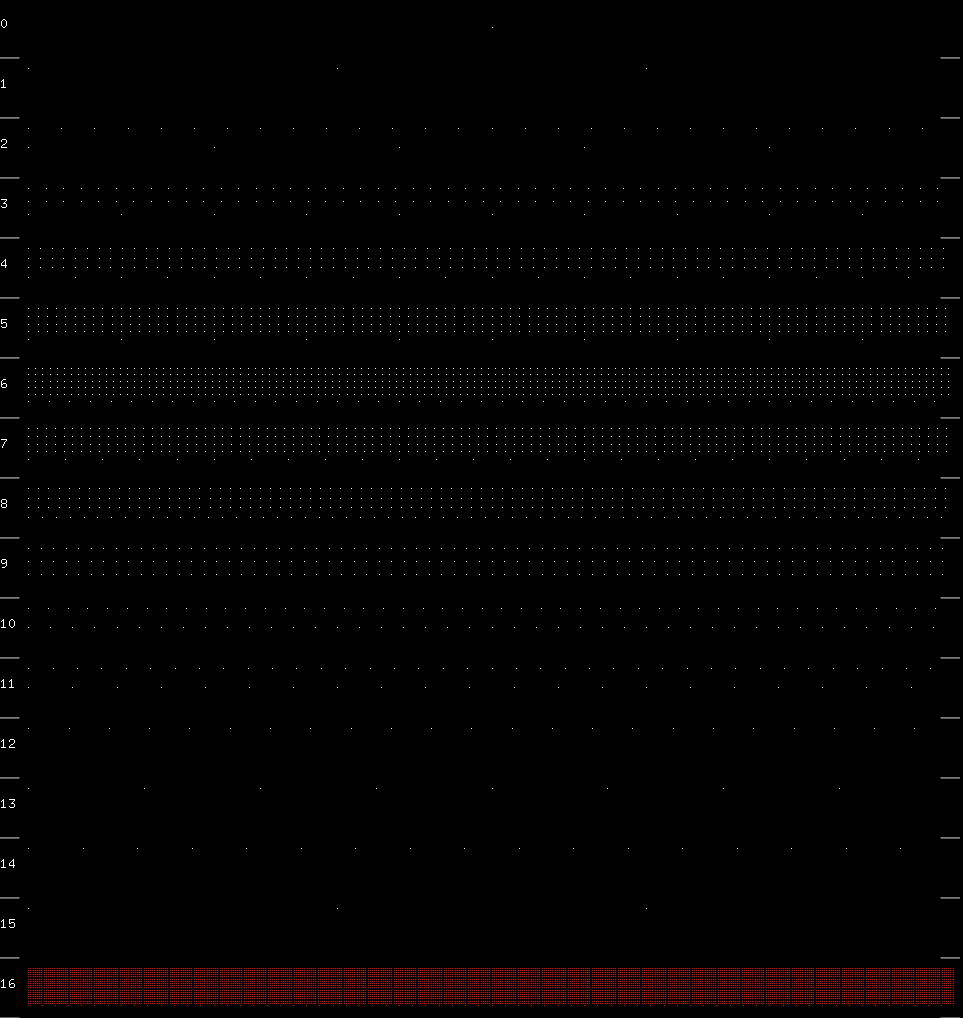
\includegraphics[scale=0.3]{pictures/go_leaves_bottom_layout.png}
\caption{Leaves bottom layout}
\label{fig:go_leaves_bottom_layout}
\end{figure}

All provided features help to improve visualization and decrees amount of element in the scene. But even with hided edges visualized sub-tree could be complicated.
The result of sub-graph highlighting is shown in Figure~\ref{fig:go_no_edge_bundling}.

\begin{figure}[h!]
\centering
\subfloat[Straight edges]{
    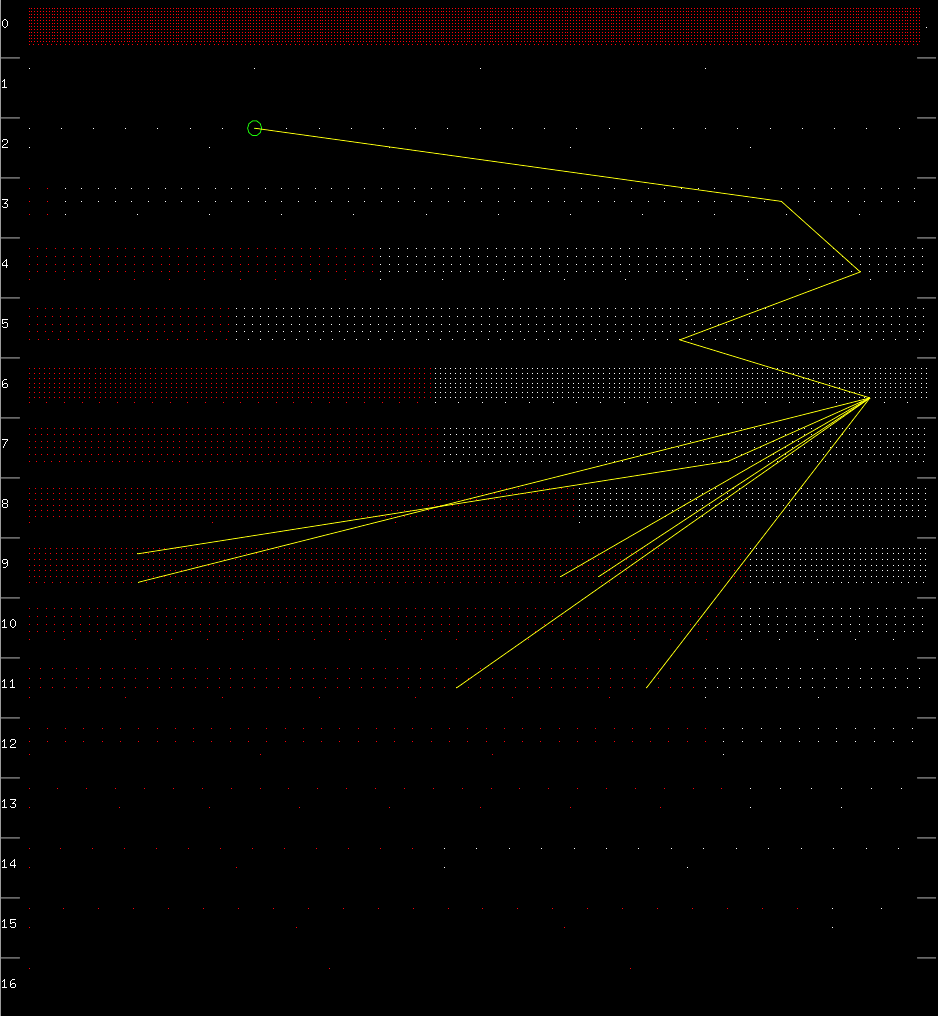
\includegraphics[scale=0.2]{pictures/go_no_edge_bundling.png}
    \label{fig:go_no_edge_bundling}
}
\subfloat[Edge bungling]{
    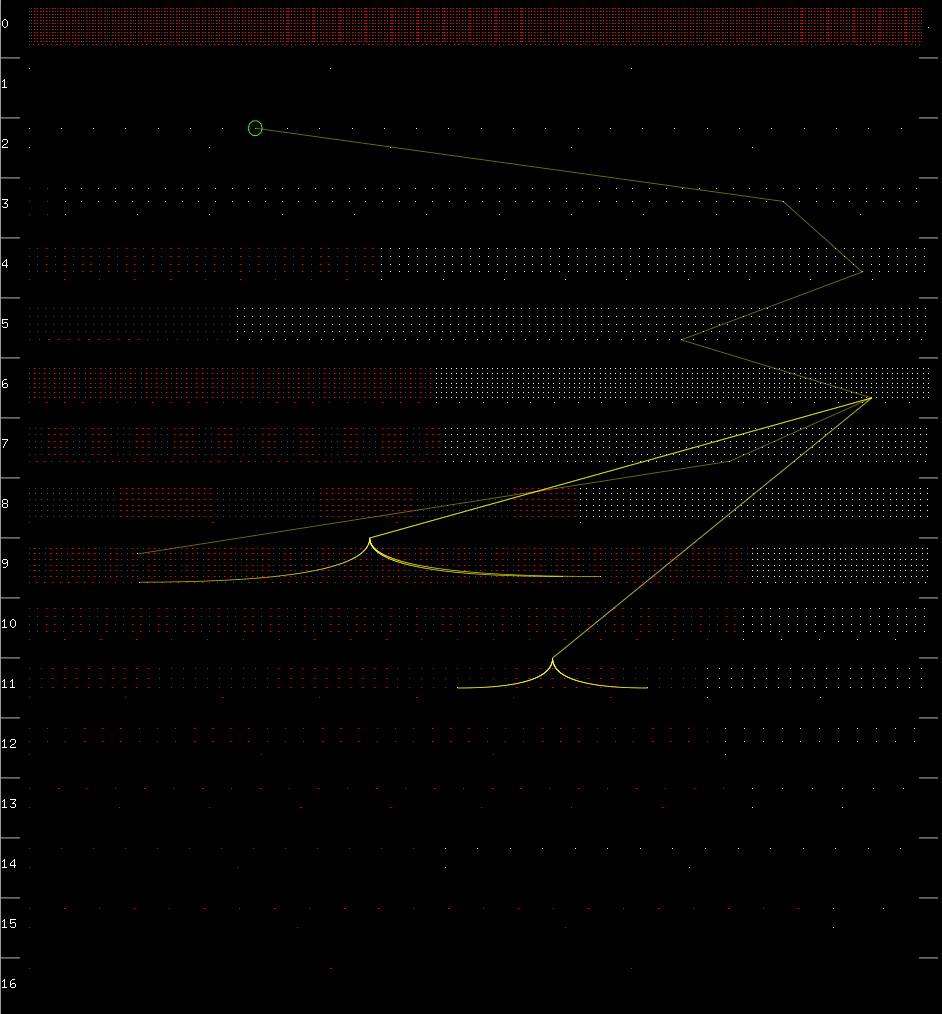
\includegraphics[scale=0.2]{pictures/go_edge_bundling.png}
    \label{fig:go_edge_bundling}
}
\caption{Gene Ontology sub-graph edge highlighting}
\label{fig:go_subgraph_highlighting}
\end{figure}

Improved edge visualization for the same selected vertex ``multicellular organismal process'' is shown in Figure~\ref{fig:go_edge_bundling}.
A newer solution is simple edge bundling. Edge bundling technique and usage example well described in the~\cite{EDGE_BUNDLING_1} and~\cite{EDGE_BUNDLING_2}.

For all edges which go into same level computed ``dummy node'' located on the top of the target level and in the middle of outlined vertices, drawing single line from source to
``dummy node'' as first part. Second part is to draw ``Bezier line'' from ``dummy node'' to target vertex. This solution helps to follow the connection and to use space in the right way.
%%%%%%%%%%%%%%%%%%%%%%%%%%%%%%%%%%%%%%%%%%%%%%%%%%%%%%%%%%%%%%%%%%%%%%%%%%%%%%%%%%%%%%%%%%%%%%%%%%%%